\documentclass[10pt]{beamer}
\usepackage[UTF8]{ctex}

\usetheme[
%sidebar, % 会在每页左侧加上导航栏,参考 The AAU Sidebar Beamer Theme 设置
xjtublue, % 不选会默认红色调,选上会将主题设置为蓝色调
% english % 选上,会将图表等标题还原回英文标题
%hidetitle,
%hideauthor,
%hideinstitute,
]{XJTUstyle}

\makeatletter
\let\@@magyar@captionfix\relax
\makeatother

\graphicspath{{figures/}}

\usepackage{array}
\usepackage{booktabs}

\AtBeginDocument{%
    \title{面向多CPU集群的\\深度行人重识别研究}
    %\subtitle{子标题}
    \author[李源勋]{%
        \begin{tabular}{ll}
            学\qquad{}生:& 李源勋 \tabularnewline
            指导老师:& 何~~~~晖
        \end{tabular}
    }
    \institute[]{西安交通大学\\计算机~44~班} % 中括号部分为导航栏底所用尽可能精简
    \date{\today}% 时间可自行设置
}
\begin{document}%

%首页标题页
\frame[plain,noframenumbering]{\titlepage}

%目录
\section*{目录}
  \frame {
    \frametitle{\secname}
    \tableofcontents[hidesubsections,sections={<1-6>}]
  }

\section{课题的任务、目的和意义}

\subsection{课题的任务}

\begin{frame}
    课题的任务
\end{frame}

\subsection{课题的目的}

\subsection{课题的意义}

\section{原始资料与相关工作}


\section{基本内容及主要方法}
\section{实验结果}

\subsection{自采集数据呈现}

\begin{frame}{数据预处理}
    \begin{block}{}
        \begin{enumerate}
            \item 视频转码
            \item 时间点校正和估计
            \item 视频切割
            \item 行人检测
            \item 人工标注
        \end{enumerate}
    \end{block}
    \begin{figure}
        \centering
        \includegraphics[width=\textwidth]{label}
        \caption{数据预处理的最终结果}
        \label{fig:label}
    \end{figure}
\end{frame}

\begin{frame}{行人检测效果}
    \begin{block}{}
        检测视频画面帧中的行人,输出bounding box。使用Facebook开源的Detectron工具,其实现了Mask RCNN框架。
    \end{block}
    \begin{figure}
        \centering
        \includegraphics[width=0.3\linewidth]{1-2_5_151.jpg}~
        \includegraphics[width=0.3\linewidth]{3-7_10_394.jpg}\\
        \includegraphics[width=0.3\linewidth]{1-2_5_151_det.jpg}~
        \includegraphics[width=0.3\linewidth]{3-7_10_394_det.jpg}
        \caption{Detectron行人检测结果可视化}
        \label{fig:detectron}
    \end{figure}
\end{frame}

\begin{frame}{自采集数据呈现}
    \begin{table}
        \centering
        \begin{tabular}{c}
            \includegraphics[width=14mm]{figures/1-1}~\includegraphics[width=14mm]{figures/1-2} \\
            \includegraphics[width=14mm]{figures/1-4}~\includegraphics[width=14mm]{figures/1-5}~\includegraphics[width=14mm]{figures/1-6} \\
            \includegraphics[width=14mm]{figures/2-1}~\includegraphics[width=14mm]{figures/2-2}~\includegraphics[width=14mm]{figures/2-3}~\includegraphics[width=14mm]{figures/2-4} \\
            \includegraphics[width=14mm]{figures/3-1}~\includegraphics[width=14mm]{figures/3-2}~\includegraphics[width=14mm]{figures/3-3} \\
            \includegraphics[width=14mm]{figures/3-4}~\includegraphics[width=14mm]{figures/3-5}~\includegraphics[width=14mm]{figures/3-6}~\includegraphics[width=14mm]{figures/3-7} \\
        \end{tabular}
    \end{table}
\end{frame}

\begin{frame}{与其它数据库的比较}
    \begin{table}
    \scriptsize
    \centering
    \caption{行人重识别领域常见数据库情况统计}
    \label{tab:reiddataset}
    \begin{tabularx}{\textwidth}{ccccccc}
    \toprule
    数据集名称   & 公布时间 & 行人数量 & 摄像头数量 & 图片数量  & Multi-shot & 跟踪 \\ \midrule
    VIPeR  & 2007 & 632  & 2     & 1264  & 否  & 否 \\[0.5em]
    CUHK01 & 2012 & 971  & 2     & 3884  & 否  & 否 \\[0.5em]
    CUHK03 & 2014 & 1467 & 10    & 13164 & 是  & 否 \\[0.5em]
    Market1501 & 2015 & 1501 & 6     & 32217 & 是  & 否 \\[0.5em]
    DukeMTMC4reID  & 2017 & 1852 & 8     & 46261 & 是  & 否 \\[0.5em]
    Multi-Cameras1 &  -   & 15   & 17     & 98543 & 是  & \textbf{是} \\[0.5em]
    Multi-Cameras2 &  -   & 463 & 24     & - & 是  & \textbf{是} \\
    \bottomrule
    \end{tabularx}
    \end{table}
\end{frame}

\subsection{行人重识别算法实现}

\begin{frame}{行人重识别算法实现结果}
\begin{block}{}
    训练阶段交叉熵误差(Loss)随着数据集训练批次数(Epoch)变化曲线如图~\ref{fig:loss}~所示。在测试阶段得到的结果与原论文中展示的结果比较如表~\ref{tab:test}~所示。
\end{block}
\begin{columns}[]
\centering
\begin{column}{0.45\textwidth}
    \vskip -1em
    \begin{figure}[]
        \centering
        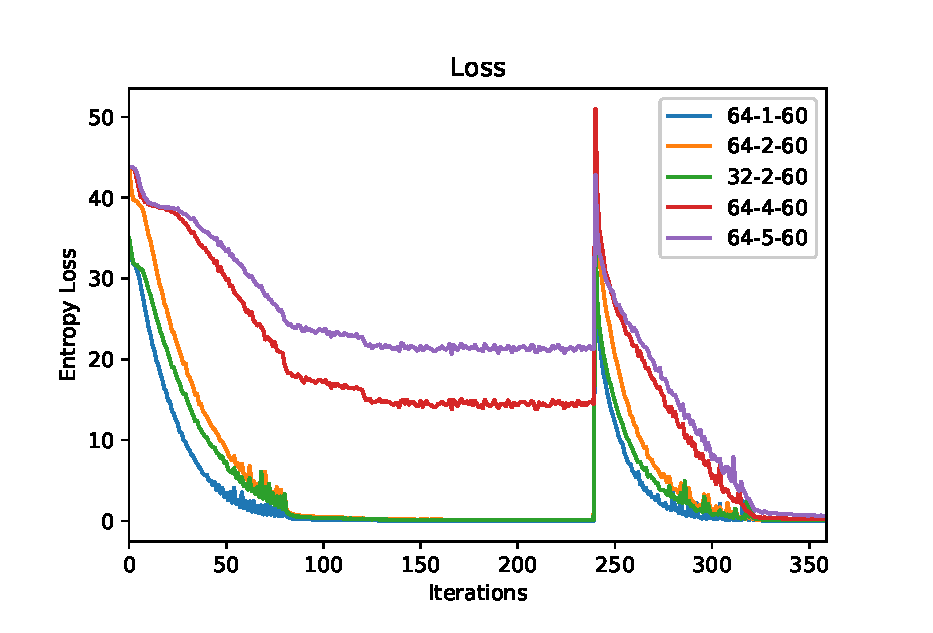
\includegraphics[width=\textwidth]{figures/loss}
        \caption{交叉熵误差随迭代数\\变化曲线}
        \label{fig:loss}
    \end{figure}
\end{column}
\begin{column}{0.5\textwidth}
    \vskip -1em
    \begin{table}
        \centering
        \scriptsize
        \begin{threeparttable}
            \begin{tabularx}{\textwidth}{p{0.2\textwidth}p{0.16\textwidth}<{\centering}p{0.16\textwidth}<{\centering}p{0.16\textwidth}<{\centering}}
                \toprule
                & mAP~(\%)   & Rank1~(\%) & Rank10~(\%) \\ \midrule
                PCB     & 77.40  & 92.30  & 98.20   \\[0.5em]
                PCB+RPP & 81.60  & 93.80  & 98.50   \\[0.5em]
                {\bf PCB}            & {\bf 73.10}  & {\bf 87.20}  & {\bf 93.40}   \\[0.5em]
                {\bf PCB+RPP}        & {\bf 74.03}  & {\bf 89.43}  & {\bf 94.40}   \\ \bottomrule
            \end{tabularx}
        \end{threeparttable}
        \caption{Market1501数据集测试结果}
        \label{tab:test}
    \end{table}
\end{column}
\end{columns}
\end{frame}

\begin{frame}{测试结果可视化}
    \begin{columns}
        \begin{column}{0.5\textwidth}
            图~\ref{fig:testvis}~是测试结果的可视化,左边一列是查询图片,每一张查询图片相应的右边一行是从测试库中挑选出来的图片,有红色边框的图片代表该人物标签与相应的查询图片人物标签不一致。
        \end{column}
        \begin{column}{0.5\textwidth}
            \begin{figure}
            \centering
            \includegraphics[width=\textwidth]{figures/vis3}
            \caption{测试结果可视化}
            \label{fig:testvis}
            \end{figure}
        \end{column}
    \end{columns}
\end{frame}

\subsection{用于多摄像头选择的强化学习模型}

\begin{frame}{经强化学习训练后的选择}
    \begin{block}

        表~\ref{tab:rlresult}~为经过强化学习训练后的智能体在应对各种状态时,最有可能采取的行动统计。图~\ref{fig:rlresult}~为最优状态的可视化。
    \end{block}
    \begin{columns}
        \begin{column}{0.5\textwidth}
            \begin{table}
                \centering
                \scriptsize
                \begin{tabularx}{\textwidth}{p{0.48\textwidth}p{0.1\textwidth}p{0.2\textwidth}}
                    \toprule
                    方案               & 频次  & 占比~(\%)  \\ \midrule
                \texttt{(1, 2, 7, 10, 14)} & 190 & 65.97 \\[0.2em]
                \texttt{(1, 2, 7, 10, 13)} & 78  & 27.08 \\[0.2em]
                \texttt{(1, 2, 7, ~9, 14)} & 18  & 6.15  \\[0.2em]
                \texttt{(1, 3, 7, 10, 14)} & 1   & 0.35  \\[0.2em]
                \texttt{(0, 2, 7, 10, 14)} & 1   & 0.35  \\ \bottomrule
                \end{tabularx}
                \caption{学习后选择的部署方案}
                \label{tab:rlresult}
            \end{table}
    \end{column}
    \begin{column}{0.5\textwidth}
            \begin{figure}
                \centering
                \includegraphics[width=0.3\textwidth]{1-2}
                \includegraphics[width=0.3\textwidth]{1-4}\\[0.3em]
                \includegraphics[width=0.3\textwidth]{2-3}
                \includegraphics[width=0.3\textwidth]{3-2}
                \includegraphics[width=0.3\textwidth]{3-6}
                \caption{最优部署方案}
                \label{fig:rlresult}
            \end{figure}
        \end{column}
    \end{columns}
\end{frame}

\subsection{分布式CPU训练}

\begin{frame}{多CPU集群分布式训练与单机的比较}
    \begin{block}

        表~\ref{tab:comp1}~展示了深度行人重识别模型分别在单机及多CPU集群上训练的时间性能。
    \end{block}
    \begin{table}
        \centering
        \footnotesize
        \begin{tabularx}{\textwidth}{X<{\centering}X<{\centering}X<{\centering}}
            \toprule
            集群节点个数 & 时间~(~s/epoch~) & 分布式开销~(~s~)~\tnote{a} \\ \midrule
            1 & 5821 & 0   \\
            2 & 3016 & 211 \\
            4 & 1536 & 323 \\
            5 & 1219 & 274 \\ \bottomrule
        \end{tabularx}
        \caption{多CPU集群分布式训练与单机的比较}
        \label{tab:comp1}
    \end{table}
\end{frame}
\section{贡献与价值}

\begin{frame}{贡献与价值}
    \begin{block}

        {\bf 1. 基线模型准确率高}
        \vskip 0.1em
        {\tiny 本文实现的行人重识别基线模型取得了接近原论文的准确率和识别性能,为后期进一步研究行人重识别领域其它问题提供了强有力的支持。}
        \vskip 0.8em

        {\bf 2. 多CPU集群的作用与潜力}
        \vskip 0.1em
        {\tiny 面向多CPU集群的深度行人重识别模型训练验证了CPU和GPU在进行海量单精度浮点数运算的性能差异,同时也展示了多CPU集群在训练深度神经网络方面的巨大潜力。}
        \vskip 0.8em

        {\bf 3. 高质量的行人重识别数据库}
        \vskip 0.1em
        {\tiny 本文推出的行人重识别数据集包含了17个摄像头,并且还包含了完整的行人跟踪场景,不仅在摄像头数量上远远多于现有主流的行人重识别数据集,而且为行人重识别问题新的评估方式的提出提供了基础。}
        \vskip 0.8em

        {\bf 4. 强化学习模型与人类认知相符}
        \vskip 0.1em
        {\tiny 本文提出的基于强化学习模型的摄像头部署方案选择模型,将强化学习算法运用到多摄像头选择问题当中,避免了穷举计算,且达到了理想的效果。}
    \end{block}
\end{frame}

%\xdbg%末页致谢
\frame[plain, noframenumbering]{\finalpage{{\huge 谢谢!}}}

\end{document}
